% !TEX root = ../main.tex
\section{Background}
\label{sec:lit}

\subsection{Physical system of stringed instruments}
\label{sec:physical-sys}
Accurate sound profile modelling of acoustic stringed instruments is a challenging problem within the digital audio effects field. A naive view of the system model may consider it as a vibrating string with specific boundary conditions imposed at the bridge and the neck of the instrument. The reality is that a complex interplay between the string, neck, bridge and body of the instrument which gives rise to the traditional acoustic timbre \cite{rossing-string-instruments}.

Non-linearities between the strings and bow, and coupling between the vibrational modes of the strings and body of the instrument via the bridge gives rise to a rich sound profile, and consequently, a detailed frequency spectrum. Each component of the instrument can be modelled in isolation, but it is the combination of each system which gives rise to the complexity.

One of the most prominent sources on bowed string modelling is Helmholtz \cite{helmholtz1862}, in which the envelope of the string is modelled produces a typical sinusoid, whilst the snapshot of the string at a point during motion produces a triangular shape with a kink when subjected to a bowing force (\ref{fig:helmholtz-string}). The peak (or trough) of this triangular string waveform is known as a "Helmholtz corner". During each cycle of the string waveform, the point of contact under the bow alternates between sticking and slipping, which gives rise to a sawtooth force waveform of the string applied to the bridge.

This is of course, in the ideal case when the bowing force is continuously applied and perpendicular to the motion of the string and does not consider more complex bowing motions.
\begin{figure}
\centering
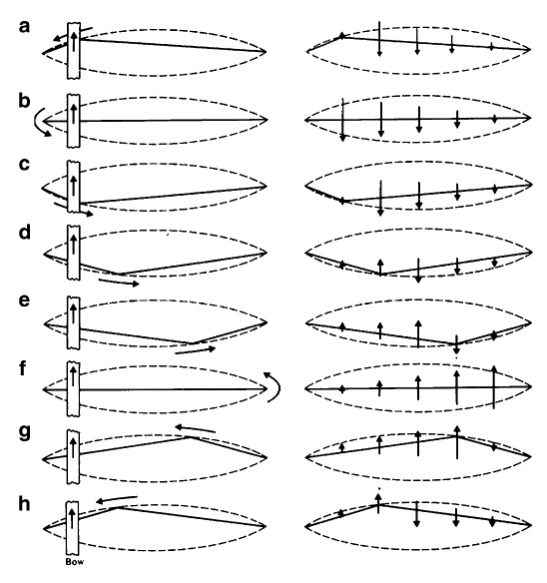
\includegraphics{figures/out/t-d-rossing-string.png}
\caption{The profile of a vibrating string when a bowing force is applied. The dashed line represents the envelope, and the solid line represents the instantaneous string shape. (from Rossing, T. \cite{rossing-string-instruments})}
\label{fig:helmholtz-string}
\end{figure}
C. V. Raman further extended the foundational work of Helmholtz by considering higher orders of discontinuities in the string velocity profile, giving rise to more complex waveforms, although still triangular in nature \cite{raman1918bowed}.

The limits of these forces exerted on the bow must feature physical limitations, and the relationship has been captured graphically by Schelleng \cite{schelleng1974}. Below the minimum bow force exerted on the string, the string will not be able to sustain the sticking required during the cycle, and exerting force above the maximum limit, the instrument will produce a "crunchy" sound \cite{woodhouse1993}.

Vibration of the instrument body due to the force exerted on the bridge by the strings will also give rise to its own set of modes, and additionally are much harder to model. Each frequency component of the vibrating body is referred to as a mode of the system, composed of the frequency, phase, amplitude and decay of the constituent sinusoid. The body itself can be broken down into its constituent components i.e., the front plate, the back plate etc., which each feature their own fundamental modes, and cannot strictly be considered in isolation.

Advances in computational methods and hardware improvements allow for more complex simulations to be performed, such as by Perez et al., in which Finite Element Modelling methods are applied to a set of six violin top plates to determine the impact of plate thickness on the first six eigenmodes of the top plate \cite{perez2023}. Despite the care taken by the authors during the manufacturing stages to select material from the same tree at the same height, there was significant variation in the elastic constant for all six plates, which would inevitably have an effect on the frequency response of the instrument. This work exemplifies the complex nature of instrument construction, and why prominent instruments, such as the Stradivari family, are so highly sought after for their tonal qualities given the difficulty involved in reproducing them.

Holographic interferometry is another powerful tool that has been utilised by Jansson et al. \cite{jansson1970} to examine the modes of the full violin body at various stages of construction. Furthermore, the frequency response of sections of the instrument may be influenced dependent on the origin of the excitation on the geometry of the piece. Fouilhe et al. explore the excitation modes of a cello tailpiece by applying an impact hammer across the front facing profile on a dead rig \cite{fouilhe2011}. While the modes of the tailpiece are examined under tension on a dead rig, an additional mass as small as 30g produces a lower frequency by approximately 9-29\%. Considering each of these components in tandem, it is apparent that the overall system is extremely complex, and accumulation of small differences in instrument parameters can have large effects on the frequency response.

\subsection{Measurement of the bridge response}
\label{sec:measurement}
Whilst the full behaviour of a bowed string instrument is composed of all of (but not limited to) the previously highlighted components, the response of the instrument body to bridge excitation is a reasonable linear, time-invariant approximation. The bridge force exerted on the body radiates sound, and this frequency response can be exploited to reproduce the sound profile of the of an acoustic instrument utilising a digital reconstruction of the frequency response \cite{karjalainen2008}.

Proper excitation of the instrument bridge is necessary to elicit the full frequency spectrum of the instrument, and sufficient energy must be imparted into the bridge to excite all the relevant modes, whilst remaining below the threshold at which it would cause damage or deformation to the soft wood of the bridge, which will in turn lead to non-linearities in the response of the system. Current literature tends to support suspending or supporting the body of the instrument via rubber bands or a stand \cite{maestre2013} with strings being damped by a soft material such as cloth or foam between the string and neck on the fingerboard, and an additional piece of foam damping the strings near the tailpiece. This reduces the impact of string vibration, typically to negligible levels.
The measurement of bridge velocity is typically performed using one of two measurement systems:
\begin{itemize}
    \item a laser vibrometer (measuring bridge velocity \cite{maestre2013}),
    \item an accelerometer (measuring bridge acceleration) \cite{woodhouse2014}
\end{itemize}
A pseudo velocity measurement can be performed utilising a contact microphone on the opposite side of the bridge to the applied force of the impact hammer, though the vibrometer method is typically preferred. This produces the bridge admittance (bridge mobility), and is necessary in the calculation of string dynamics modelling\cite{maestre2013}.

Under the same experimental setup, the bridge acoustic pressure can be measured utilising a single, or multiple microphones, as explored in \cite{maestre2019}. As sound radiates in 3D space from a source, Maestre et al. highlights the complexity of modelling this problem. Dominant frequency components will vary according to the direction that the sound is recorded from (or listened to), providing another layer of complexity, referred to as directivity. Maestre attempts to model this utilising an array of 60 microphones surrounding a violin and clarinet. The transfer function of the cello body features high modal densities, and as noted in \cite{oneill}, an adequate sound profile and frequency domain approximation required approximately 2000 parallel filters for satisfactory reconstruction.
% INSERT SECTION ABOUT TRANSFER FUNCTION RECORDING AND ADMITTANCE MEASUREMENTS

Obtaining a representation of the bridge admittance follows a similar process, in which the bridge of the system is again excited by an impact hammer but the oscillation of the bridge velocity is measured, as opposed to sound pressure. Bridge velocity is a much lower modal reconstruction order.

The modelling of the impulse response that arises from the excitation of the instrument bridge, and the associated frequency response is the focus of this work.

\subsection{Modal analysis and spectral estimation}
\label{modal-analysis}
The approach of approximating a complex system as linear, given suitable boundary conditions, is ubiquitous across engineering and physics. The approach offers several notable benefits, one of which is the linear independence of the eigenvectors of the system, or fundamental modes. A more detailed treatment of the full modal analysis can be found in \cite{modal-analysis-violin}.

By decomposing the system into a set of composite waveforms, an elegant formulation which yields the fundamental frequencies, damping factor and fundamental modes of the instrument can be recovered via the system poles \cite{juang-1994-book}. Whilst an attractive approach, recovery of the modes themselves is difficult due to the introduction of measurement noise into the system. Several methods have been developed in an attempt to rectify this.
% 3rd point - Survey of methods
A fundamental limitation of non-parametric methods, such as the Discrete Fourier Transform as a frequency domain analysis tool is the inability to represent multiple modes at the same frequency and modes which are tightly spaced in the frequency domain, being gated by the frequency resolution $\frac{1}{N\tau}$. In the context of stringed instruments, modal density is high and the modes can additionally be closely spaced or overlap, thus exemplifies why the DFT is insufficient in isolation as an analysis tool. Parametric methods, such as Autoregressive Moving Average (ARMA), Multiple Signal Classification (MUSIC) and Estimation of Signal Parameters via Rotational Invariance Techniques (ESPRIT) make some underlying assumptions about the form of the data \cite{music, esprit}.

ARMA modelling represents the signal as a pole-zero filter driven by noise and estimates the model coefficients to obtain a super-resolution spectral estimate.As the estimation is non-linear, it becomes difficult to accurately calculate modes at higher model orders for systems with closely spaced modes \cite{hayes}.

MUSIC is a subspace based method typically applied in array processing to determine the direction of arrival estimation. The model assumes that the signal is composed of a multitude of complex exponentials embedded in gaussian noise. The algorithm assumes that the sinusoids span a signal subspace, and the remaining noise subspace is orthogonal to the signal subspace. It should be noted that MUSIC produces a pseudo-spectrum and not a true power spectrum, and thus it is typical that an additional frequency analysis method to determine dominant modes, such as peak finding applied to the pseudo-spectrum must be applied before the frequencies are then modelled. The frequency grid over which the algorithm searches can be arbitrarily defined depending on the application, thus giving rise to the super-resolution property of this method. As noted in \cite{music1986}, the performance of the algorithm can degrade in the presence of noisy signals.

ESPRIT also separates signal and noise subspaces via eigendecomposition, but instead of exploiting a grid search, recovers the signals directly. It is based on the rotational invariance between two time shifted copies of the signal subspace and the eigenvalues of the matrix relating the two copies provide the frequencies of the system modes. The short fall of both base MUSIC and ESPRIT is that they do not account for damping in the system, instead assuming that the signals are pure sinusoids, similar to the DFT.
Although these methods yield a loss of generality, they become a much more powerful analysis tool in describing the underlying behaviour of the signal by providing greater resolution. A direct consequence of this assumption is that inappropriate application of parametric methods can produce misleading or meaningless results in the event the model is a poor match for the signal under investigation \cite{hayes}.

Several applications of these methods in the context of modal parameter extraction have been applied \cite{mode-extraction}, all of which are included in the Matlab Vibration Analysis toolbox.

% Write a little bit about FDM in here.
The basis for this project will be an extension of the work explored in \cite{dafx2026}, and a comparison with the method applied in by O'Neill in \cite{oneill}. O'Neill applies the Filter Diagonalisation Method (FDM) \cite{fdm} to the cello body transfer function, which is comprised of a large number of modes, and utilises the modal parameters produced (frequency, amplitude, phase and decay) to compose a set of IIR filter coefficients via the impulse invariant method.

% Maybe I need to speak to Dr. van Walstijn about the rejection methods here, I'm asserting this claim with no source?
There are several challenges in the utilisation of the FDM method, notably the modal density of the cello body transfer function, the degree of manual tuning of the rejection thresholds necessary for each modal parameter and the computational time associated with applying the FDM. Whilst the method is computationally expensive, the resulting application has received positive feedback on its sound profile from a professional cellist when applied to a 3D printed cello system, and visually approximates the true cello body frequency response function well. Additionally, the significance of the phase of the frequency response has been highlighted, alongside the ability to dynamically adjust the decay rate when the filters are applied to a 3D printed cello system which generates an output by convolving the applied input with the parallel filter bank coefficients generated via an audio plugin in real time.

\subsection{The Eigensystem Realisation Algorithm}
To explore alternative methods with reduced computational complexity and the possibility of algorithm based spurious mode rejection, the Eigensystem Realisation Algorithm (ERA), originally outlined by Juang and Pappa \cite{era,era-space} for use in structural modal analysis is implemented and investigated.
Ho and Kalman first introduced the concept of the minimum realisation problem is "equivalent to a representation involving a sequence of real matrices known as Markov parameters" \cite{era}. A minimum realisation is the smallest number of dimensions across the state space representation which can describe the input and output relationship of the system to the degree of accuracy required, i.e., a minimal approximation of the true system representation. ERA builds on the work carried out by Ho and Kalman, introducing a singular value decomposition (SVD) stage to truncate the order of the system. Given that noise and signal subspaces are orthogonal, the $\Sigma$ matrix can be truncated to effectively remove the noisy part of the signal in question. The benefit of ERA as opposed to other parametric methods is its ability to deal with damped modes, and clean mode order selection via SVD truncation, allowing a simple and efficient reconstruction of the impulse response of the system.
Whilst ERA has been applied extensively in other areas of engineering \cite{pappa1998,lin2021,zhang2016,chiang2010}. The full derivation of the ERA can be found in Section \ref{sec:era-proof}.

Whilst the mathematical implementation of ERA is elegant, real world applications are never so clean and simple. Real world signals carry noise and imperfections in the recording. For example, recording the radiated sound pressure from the excitation of the instrument bridge may introduce acoustic reflections from the walls of the room \cite{haasjes2024}, in addition to the instrument noise inherent to measurement equipment.

% Really need to maybe have a discussion of this section with Dr. van Walstijn, the scope of the project did change imo.
There are a multitude of methods that have been applied to ERA to combat artefacts and non-physical modes introduced in the decomposition process, including Modal Amplitude Coherence (MAC) and Modal Phase Collinearity (MPC), Mode Similarity Index (MSI) and Singular Vector Smoothness (SVS). MAC and MPC require multiple measurements of the signal at different geometric locations, and MSI and SVS were lightly explored, but deemed too require too much tuning of hyper-parameters to explore further in the timeframe of the project \cite{caicedo2010, uradnicek2025, zhang2014, chen2020}. Two primary methods are applicable in a single-input-single-output (SISO) system:
\begin{itemize}
    \item Singular value spectrum: By examining the singular values of the SVD decomposition of the Hankel matrix, this may provide a visual indicator of the singular value cut-off point between the signal and noise subspace.
    \item Stabilization Diagrams: These diagrams iterate over the eigensystem realisation for various mode orders to determine which modes are consistent throughout the model. Stable, physical modes will repeatedly appear across all model orders.
\end{itemize}

ERA is well-established method applied in structural dynamics contexts, but has only recently explored in the application of string instrument admittance and radiated acoustic pressure \cite{dafx2026}. This work explores ERA as a reduced computational complexity alternative to FDM with a direct comparison.
The report is structured as follows: Section \ref{sec:mathematics} covers the mathematical background of ERA and subsequent IIR filter formulation, Section \ref{sec:validation} validates the algorithm development on clean and noisy signals, Section \ref{sec:measurements} details the measurement of cello body signals and post-processing applied to both bridge admittance and cello body signals, Section \ref{sec:results} details the resultant modal fitting, and Section \ref{sec:discussion} discusses these results.
% Overall, there is potential for ERA to offer similar performance to the FDM method for parametric convolution, with the additional benefit of a reduced burden on manual intervention when analysing the modes and accompanying FRF to reproduce desirable modal profile.